\chapter{Lektion 4}

\section{Kapitel 8}

Hvis man vil undgå at ens produkt går mod ligevægt og man ikke længere får et stor overskud skal man have \textbf{copyright}. Dette bliver så til et ikke fuldkomment konkurrerende marked, eller et prissætte marked. 

\subsection{Perfect and imperfect competition}
Økonomer adskiller for det meste mellem tre forskellige typer af ikke fuldkomne markeder. 

\subsubsection{Different forms of imperfect competition}

Længst fra fuldkommen konkurrence er rent monopol. Hvilket er hvor der kun er en sælger på markedet. 

\textbf{Monopolistic competition}: Det er et marked hvor mange rivaler sælger et produkt der er tæt på hinanden, men ikke helt perfekte substitutter. Der er altid en eller anden ting ved hvert produkt der gør at nogle kunder ville foretrække varen. Det har en ting til fælles med fuldkommen konkurrence, hvilket er at man kan komme og gå fra markedet som man vil. Et eksempel på monopolistisk konkurrence er lokale olieselskaber, her er produktet egentlig det samme men placeringen for tanken spiller en stor rolle for forbrugeren. Hvis kunderne foretrækker en vare frem for en anden kan producenten hæve prisen en smule uden at miste nogen kunder. Dette betyder dog ikke at firmaet vil opleve økonomisk profit på lang sigt. Hvis andre firmaer kunne se at der var profit i markedet ville de komme ind på det, og selv om de ikke ville kunne producere det præcis samme vare ville prisen stadig presses ned. Dette vil ske da andre måske ser større fordele i det nye produkt og derfor vil de gamle miste kunder. Altså vil firmaerne i markedet igen ende med en økonomisk profit på 0.

Indenfor denne markedstype skal producenterne ikke bare vælge prisen med omhu men også varen. Hvor meget skal den afspejle en anden vare?

\textbf{Oligopoly}: Mellem fuldkommen konkurrence og monopol ligger oligopol, hvilket består af få store firmaer. Ligesom monopol er oligopol tit en konsekvens af omkostningsfordele, der forhindre mindre firmaer i effektivt at konkurrere. Under oligopol sælger producenterne tit det samme produkt, fx cement. Firmaer der er på et marked der er under oligopol, skal fokusere på prissætningen og reklamen frem for produktet. Omkostningsfordele tilknyttet store størrelser er for det meste vigtigt under oligopol, og det vil helt klart gøre at adgang og at forlade markedet vil gøre at den økonomisk profit er 0. Det er ikke sikkert at selvom at to firmaer på et oligopol marked har et økonomisk overskud at hvis en tredje træder ind i markedet at det også vil have overskud, eller måske alle tre nu vil have underskud på grund af en lavere pris. 

Fra nu af vil en fra et af de tre ikke fuldkomne markeder kaldes en monopolist i dette kapitel.

\subsubsection{The essential difference between perfectly and imperfectly competitive firms}

\textit{Firmaer i fuldkommen konkurrence står med en perfekt elastisk efterspørgselskurve for deres produkt, hvorimod firmaer i ikke fuldkommen konkurrence står med en efterspørgselskurve med en negativ hældning.} Der er en ligevægtpris på det fuldkomne marked der ikke giver nogen mening at afvige fra da det er der de sælger alle deres varer. Derfor er efterspørgselskurven en horisontal linje. Hvis et firma i ikke fuldkommen konkurrence derimod sætter prisen lidt op, er det ikke sikkert at det er alle der forlader "ham", og derfor har efterspørgselskurven en negtiv hældning. 

\subsection{Five sources of market power}
De firmaer der har en efterspørgselskurve med negativ hældning siges at nyde markeds krafterne, som referer til deres mulighed om at ændre priserne. Eksklusiv kontrol over inputs, patent og copyright, offentlige licenser, stordriftsfordele og netværksøkonomier er 5 ting der gør at konkurrencen bliver begrænset og det dermed er muligt at nyde markeds krafterne. 

\subsubsection{Exclusive control over important inputs}
Hvis et firma kontrollere et essentielt input til en vare har det firma markeds kraften. Fx mange vil betale meget for et kontor i USAs højeste bygning. Ejeren af WTC har markeds kraften.

\subsubsection{Patents and copyright}
Hvis man har patents eller copyright på noget er man den eneste der må tjene på det og derfor udelukker det andre fra at producere varen. Fx. medikamenter. 
\subsubsection{Government licenses or franchises}
Temmelig meget argumentet ovenfor.

\subsubsection{Economies of scale and natural monopolies}
Hvad sker der når et firma fordobler alle faktorerne i produktionen? Hvis output fordobles, siges produktions processen at være konstant vender tilbage til skala. Hvis output mere end fordobles sige produktions processen at have stigende vender tilbage til skala. I begge tilfælde vil den gennemsnitlige omkostning falde når produktionen stiger. Et monopol som resultat af stordriftsfordele kaldes naturlig monopol.

\subsubsection{Network economies}
Populariteten af en vare kan også afhænge af hvor mange der har varen. Hvis der er to forskellige varer, men der er en af dem der har noget der er en smule mere attraktiv, køber folk den. Selv hvis vare to formår at få den samme ting, vil folk allerede have valgt en ting, og dermed er der bedre muligheder for at tilgå denne vare, få den repereret mm. Der er fx Microsoft, selvom der måske er et brand der kan det samme, er det nemmere af få det andet og man har formentlig allerede andet der kan arbejde sammen med brandet. Det er dog ikke altid at man bare kan antage at fx. Microsoft forbliver ene på markedet, det har man kunne se de seneste år mht Apple. Netværksøkonomier, er en naturlig kilde til monopol. 

\subsection{Economies of scale and the importance of start-up costs}
Variable omkostninger af output, det gør faste omkostninger ikke, og der er ingen faste omkostninger på langt sigt da alle input kan varieres. Dog er der nogle ting hvor opstarts omkostningerne koster meget, og har en meget lav marginal omkostning. Dette kan fx være et software firma, hvor det kræver meget i starten at skrive koden, men når det er færdigt er resten billigt at "producere". Disse firmaer er underlagt betydelige stordriftsfordele, da de gennemsnitlige totale omkostninger vil falde når produktionen stiger, ATC = (fasteomkostninger / antal producerede) + marginal omkostningerne.

\begin{eks} \textbf{} %Nyt eksempel
\newline
Nintendo og Sony har begge faste omkostninger på 10.000.000 og en marginalomkostning på 0.20 per spil. Nintendo producerer 1 mio units og Sony producere 1.2 mio units.  

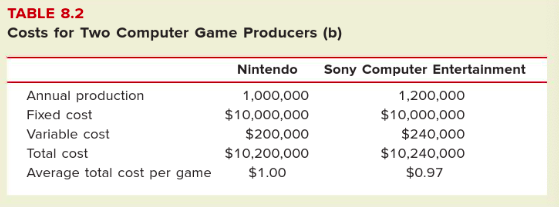
\includegraphics[scale=0.8]{Afsnit/Lektion4/Nintendoogsony.png}

Det ses her at Sony vil have mulighed for at sætte prisen lavere end Nintendo, og hvis man antager at der ikke er andet end prisen der adskiller de to, vil det gøre Sony noget mere populær end Nintendo. For at Nintendo kan sætte prisen ned skal de producere mere, så deres gennemsnitlige totale omkostninger falder. 
\end{eks}

\subsection{Profit maximization for the monopolist}
Så længe fordele overskrider omkostningerne vil firmaer producere mere, altså de marginale fordele der stiger for hver producerede vare kaldes \textbf{marginale indtægter.} De marginale indtægter for at firma i fuldkommen konkurrence er lig markedsprisen 

\subsubsection{Marginal revenue for the monopolist}
\textit{For en monopolist, er de marginale fordele ved at sælge en ekstra unit lavere end markedsprisen. } Forskellen for firmaer under fuldkommen konkurrence og monopolister, er at underfuldkommen konkurrence kan firmaer sælge alle de units de vil til markedsprisen hvor monopolisterne skal sætte prisen ned for at sælge mere.

\includegraphics[scale=0.8]{Afsnit/Lektion4/marginalindtægt.png}

På grafen se at ved at sælge 2 units, vil firmaet tjene $2 \codt 6 = 12$ og ved 3 units, vil de tjene $3 \cdot 5 = 15$. Altså er de marginale indtægter $3$. I ovenstående eksempel ses det også at den marginale indtægt vil være faldende og når den er lig nul. Hvis efterspørgselskurven skærer andenaksen i a, vil marginal indtægten være nul ved $\frac{a}{2}$ eller hvis den skærer med førsteaksen i b vil marginal indtægten være nul ved $\frac{b}{2}$. Altså hvis eftspørgselskurven kan beskrives ved $D = a - qb$ så er kurven for marginalindtægten $MR = a - 2qb$. 

\subsubsection{The monopolist's profit-maximizing decision rule}
\textit{Profitten er maksimeret på det niveau af output hvor marginal indtægten er præcis lig marginal omkostningerne}. Ved denne definition kan vi se at fuldkommen konkurrence er et specialtilfælde af monopol reglen. Når firmaer i fuldkommen konkurrence udvider med en unit, vil marginal indtægten være lig markedsprisen, fordi de kan udvide salget ved at sænke prisen af de eksisterende units. Så når firmaer i fuldkommen konkurrence sidestiller prisen med marginal omkostningerne, sidesætter de også marginal indtægten med marginal omkostningerne. \textit{Den eneste signifikante forskel mellem de to sager vedrører således beregning af marginale indtægter}

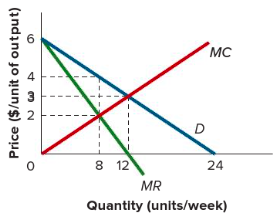
\includegraphics[scale=0.8]{Afsnit/Lektion4/maksimeringafprofit.png} \label{marginalindtægt}

Ovenstående graf viser marginal omkostningerne, efterspørgslen og marginal indtægten. Her ses det at profitten maksimeres når der sælges 8 units om ugen. 

\subsubsection{Being a monopolist doesn't guarantee an economic profit}
Selvom profit maksimerings prisen altid er over marginal omkostningerne, betyder ikke nødvendigvis ikke at der er økonomisk profit. Det sker hvis de gennemsnitlige totale omkostninger er højere end prisen hvor marginal indtægterne er lig marginal omkostningerne. Hvis de gennemsnitlige totale omkostninger er lavere en prisen hvor marginal indtægterne er lig marginal omkostningerne er der økonomisk profit. Nedenstående grafer viser et firma med henholdsvis økonomisk tab og profit. 

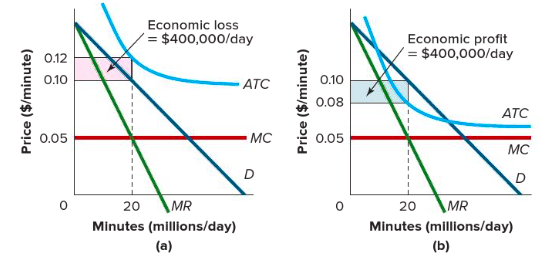
\includegraphics[scale=0.6]{Afsnit/Lektion4/tabogprofit.png}

\subsection{Why the invisible hand breaks down under monopoly}
Er maksimering af profitten det mest effektive for samfundet? Hvis vi ser på grafen i \autoref{marginalindtægt}, ved profitmaksimering ved 2 units vil en stigning med en unit gøre at marginal fordelen stiger med 4 og på det tidspunkt er marginal omkostningerne kun 2, 4-2=2, altså vil samfundet have godt af en stigning med en unit. Da dette ikke gøre er markedet ineffektivt. Monopolististen hæver ikke produktionen da det ikke altid er muligt at holde prisen på de eksisterende units, og kun sænke prisen for den ekstra unit. 

For at opnå social effektivitet, skal monopolisten hæve produktionen indtil marginal fordelene til samfundet er lig marginal omkostningerne, hvilket på figuren er 12 units, altså der hvor efterspørgsel og marginalomkostningerne skærer. 

Det at marginal indtægten er under prisen for monopolisten resultere i \textbf{dødvægts tab}. Det beregnes ved arealet af trekanten under. 

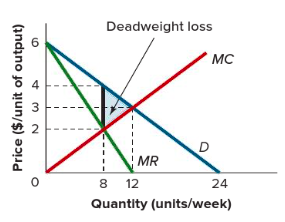
\includegraphics[scale=0.7]{Afsnit/Lektion4/trekantensareal.png}

Da fuldkommen konkurrence er effektivt, men monopol ikke er burde ting som patent så være ulovligt. Nej, det ville dræbe innovation, hvilket også styrker et samfund mm. 

\subsection{Using discount to expand the market}
Da monopoly er ineffektiv betyder det at man kunne gøre noget bedre for nogen uden at skade andre, alle kan få et større stykke af kagen. Hvorfor sælge en monopolist ikke bare itl en pris til nogen og når dem der vil give den pris har købt sætter han prisen ned?

\subsubsection{Price discrimmination defined}
Det gør nogen! Nogen betaler en pris andre en anden, dette er \textbf{prisdiskrimination}, fx seniorrabat. Nogen markeder virker det, andre gør det ikke. 

\subsubsection{How price discrimination affect output}
Hvordan påvirker prisdiskrimination monopolistens profit maksimering? 

\textbf{Perfekt diskriminerende monopolist} betyder at monopolisten tager præcis køberens reservationspris for en vare. Ved at gøre dette vil det totale økonomiske overskud være maksimeret ift hvis man ikke prismaksimerer. Dog vil kunder ikke være særlig glade for at handle med et sådan firma, da deres økonomiske overskud altid vil være 0. Perfekt diskrimination, vil heller aldrig ske da ingen sælger kender alle købernes reservationspriser. Dog er ikke perfekt pris diskrimination muligt. 

\subsubsection{The hurdle method of price discrimination}
For at maksimere profitten vil alle sælgere altid gå efter at sælge til højeste pris en køber vil give. To ting forhindre sælgeren i at gøre dette. Først er der det at sælgeren aldrig helt ved hvad køberen vil give og andet er at de har brug for nogle midler til at forhindre købere med høj reservationspris i at købe til en lav pris. \textbf{Hindringsmetoden til pris diskrimination} løser begge disse problemer ved at køberen skal overvinde en hindring for at være berettiget til rabat. Fx. man skal sende en rabatkupon på mail for at få rabat. \textbf{En perfekt hindring} er når købere præcis bliver inddelt i grupper med deres reservationspris, men det eksistere ikke rigtig. 

\subsubsection{Is price discrimination a bad thing?}
Både sælgers og det totale forbruger overskud vil være det samme eller højere hvis der er pris diskrimination. Dette sker da man ved prisdiskrimination tit oplever at dem der normalt ikke vil købe, køber under pris diskrimination, og da deres reservationspris ikke altid er det samme vil der være nogen kunder der oplever et overskud. Hvis man ligger dette overskud oveni det der tjenes fra dem der altid betale fuld pris, stiger det totale overskud(se eks fra s. 223-225. Da begge parter oplever en fremgang gør pris diskriminationen mere effektiv end bare at kræve én pris fra alle. 

\subsubsection{Examples of price discrimination}
Hindringer er fx black friday, eller bare andre perodiske rabatter, hvor hindringen her er at finde tiden og stedet hvor rabatten finder sted, og prioritere at tage tid til at tage derhen. Andre eksempler er antallet af tilbehør i en ny bil, om en bog er i hard cover eller bare en papirudgave eller om man flyver buisness eller economy. 

\subsection{Public policy toward natural monopoly}
Ved monopol bliver markedet meget mindre effektivt, og da sælgeren oplever et økonomisk overskud på bekostning af forbrugerne. Mange forbrugere har det derfor heller ikke helt godt med at købe fra en monopolist. Regeringer prøver steder at kontrollere monopolisterne på den ene eller anden måde. nogle tager styringen over monopolet og andre prøver at lave love for at kontrollere priserne, men disse politikker skaber økonomiske problemer i dem selv. Så det gælder om at komme op med en måde at skabe størst muligt overskud af fordele over ulemper. 

\subsubsection{State ownership and management}
Monopol er ineffektiv da maksimerings prisen altid er større end marginalomkostningerne. Da monopol er defineret som stordriftsøkonomier, hvor marginalomkostningerne altid er under de gennemsnitlige totale omkostninger, vil det at sætte prisen lig marginalomkostningerne ikke kunne dække de totale omkostninger. Dette resulterer i et tab. En måde at forbedre effektiviteten på er at regeringen tager over industrien, sætter prisen lig marginalomkostningerne og tager skattepenge til at finansiere tabet. Problemet ved dette er at hvis en privat monopolist skærer i omkostningerne med 1kr, stiger profitten med 1kr. Hvis en offentlig monopolist skærer i omkostningerne med 1kr, skærer de i budgettet for monopoliet med 1kr. 
\subsubsection{State regulation of private monopolies}
Hvis regeringen ikke køber hele markedet kan de anvende cost-plus reguleringer. Dette betyder at regeringen går ind sætter prisen for hver monopol så det dækker omkostningerne plus en mark-up så de er sikre en normal tilbagevenden af deres investeringer. 

\textbf{Pitfalls:}
\begin{itemize}
    \item Det er svært at bestemme hvilke af firmaets udgifter der skal inkluderes i det prisen skal dække. 
    \item Firmaer har ingen grund til at finde på ting der kan sænke omkostningerne da de er sikre på at få dem tilbage. Måske vil de endda hæve omkostningerne pga. markuppen. 
    \item Det løser ikke problemet om at vi gerne vil sætte prisen lige marginal omkostningerne. 
\end{itemize}

\subsubsection{Exclusive contracting for natural monopoly}
En af de bedste metode er at regeringen inviterer private firmaer til at byde på monopol markedet. Regeringen siger hvilket marked det handler om og hvor meget de vil betale for en service, så vinder den lavest bydende. Her vil firmaer stadig være interesseret i at mindske omkostningerne, byde-rundten gør at det er så fair som muligt mht til profitten og hvis regeringen giver penge til de vindende kan prisen sættes til marginal omkostningerne. Denne mulighed er kun mulig ved simple ting som fx skraldemænd og brandmænd, ellers kan det kræve meget komplekse investeringer i kapital.

\subsubsection{Vigorous enforcement of antitrust laws}
I 1890 blev det gjort ulovligt at lave en sammensværgelse om at "lave monopol eller forsøge at lave monopol", som fx Rockefellers. I 1914, ville de forebygge at firmaer arbejdede samme om at danne monopol. Disse \textbf{antitrustlove}, hjælper med at forhindre karteller eller firmaer i at hæve prisen. De fremmer også konkurrencen, men gør også at det ikke er muligt at blive en stordriftsøkonomi. 

\textbf{Til sidst er der den mulighed at man bare kan lade monopolet være et monopol.} For det meste sættes prisen ikke fuldstændig åndssvagt højt, og meget af den profit monopolet tjener skal alligevel betales tilbage i firma skat mm. 









